\section{Instrumentation statique}

\subsection{La problématique}

La problématique de cette partie était de dresser un profil statique du code considéré, c'est-à-dire obtenir une trace des accès mémoire à la compilation. Un exemple est illustré en figure \ref{fig:static_result}.

\begin{figure}[here]
  \centering
\begin{verbatim}
 fonction toto
 3 load
 2 * N load
 1 * N store
 2 load
 3 * M load
 3 * M store
\end{verbatim}
  \caption{Résultat obtenu par l'instrumentation statique}
  \label{fig:static_result}
\end{figure}

\subsection{Accès mémoire}

Ces accès mémoire se traduisent par les instructions load et store exécutées. Nous considérons qu'une instruction load est détectée lorsque le contenu d'un tableau est affectée à une variable, un store lorsqu'un tableau récupère la valeur d'une variable.\\

\subsection{Blocs de base et boucles}

L'idée était donc de parcourir les blocs de base composant chaque fonction du code. La principale difficulté de cette phase de profiling consistait à détecter les éventuelles boucles présentes au sein d'une fonction, puis traiter les blocs de base, en évitant les redondances.

\subsection{Parsing des boucles et blocs de base}

Cette opération a été effectuée en deux passes: le parsing des boucles \verb#pass_loop#, puis celui des blocs de base courants \verb#pass_bb#.\\

Dans les 2 passes, l'instrumentation se déroule de la façon suivante:\\

\begin{itemize}

\item La fonction principale de la passe parcourt tous les blocs de base à l'aide de la macro \verb#FOR_EACH_BB#. Puis, elle utilise un itérateur pour analyser les ``statements'', c'est-à-dire les lignes du bloc de base courant. Ceci est fait grâce à la fonction \verb#read_stmt()#.\\

\item La fonction \verb#read_stmt()# qui est appelée permet de savoir si le statement correspond à un appel de fonction, un retour, une condition, ou plus simplement une affectation\footnote{voir ``GIMPLE\_ASSIGN'' dans gimple}. C'est ce dernier cas qui nous intéresse.\\

\item Ensuite, nous avons besoin de savoir de quel côté de l'égalité nous sommes. La fonction \verb#read_stmt()# nous donne également la position de l'opérande (à droite ou à gauche de l'égalité). La fonction \verb#read_operand()#, quant à elle, détermine le type rencontré, en l'occurence, celui qui nous intéresse\footnote{voir ``INDIRECT\_REF'' dans gimple}. Un exemple de code est fournit en figure \ref{fig:count_example}.\\

\item Lorsque ce cas est rencontré, on incrémente le compteur de loads si l'opérande est à droite de l'égalité, et le compteur de stores si l'opérande se trouve à gauche.\\

\end{itemize}

\begin{figure}[here]
  \centering
\begin{verbatim}
case INDIRECT_REF:
  /* pointer & dereferencing */
  if ( store == true ) { basicblock->nstore++; }
  else { basicblock->nload++; }
  break;
\end{verbatim}
  \caption{Exemple de code d'incrementation des compteurs de load et store}
  \label{fig:count_example}
\end{figure}

\subsection{La passe des boucles}

La première passe \verb#pass_loop# détecte les éventuelles boucles présentes dans la fonction instrumentée, en la parcourant. Elle stocke dans une structure les blocs de base contenus dans lesdites boucles.\\

La détection des boucles est possible grâce au code présenté en figure \ref{fig:pass_loop}, au sein de la fonction \verb#pass_loop()#.\\

\begin{figure}[here]
  \centering
\begin{verbatim}
if ( cfun->x_current_loops != NULL )
{
    read_loop( cfun->x_current_loops->tree_root, function );
}
\end{verbatim}
  \caption{Appel de la fonction read\_loop}
  \label{fig:pass_loop}
\end{figure}

La fonction \verb#read_loop()# permet de connaître les bornes des boucles rencontrées dans la fonction, et ainsi de multiplier le nombre des opérations éventuelles load et store par le nombre d'itérations de la boucle. Les blocs de base contenant ces boucles sont écartées du traitement classique des blocs, afin d'éviter des redondances.

\subsection{La passe des blocs de base}

La seconde passe \verb#passe_bb#, quant à elle, reparcourt les blocs de base de la fonction, et vérifie pour chaque bloc considéré s'il a déjà été traité dans la passe précédente. Dans ce cas, elle passe au bloc de base suivant. Dans le cas contraire, elle analyse chaque statement du bloc.

\subsection{Localisation des passes}

Au niveau de l'enregistrement de la passe \verb#pass_loop#, nous avons changé le paramètre ``mudflap2'' dédié au parcours GIMPLE, par ``parloops''.

\subsection{Paramètres d'optimisation}

Enfin, pour prendre en compte les boucles du code à compiler, les options d'optimisation ``-O1'' ou ``-O2'' de gcc doivent être utilisées.

\subsection{Graphe CFG}

Nous vous présentions précédement les blocs de base ainsi que les ``chemins'' entre blocs de base que ``myproof'' reconnait.\\

Il nous est donc possible de générer des graphes CFG\footnote{Grammaire non contextuelle}.\\

Nous vous présentons en figure \ref{fig:cfg} un exemple de graphe d'une fonction.

\begin{figure}[here]
  \centering
  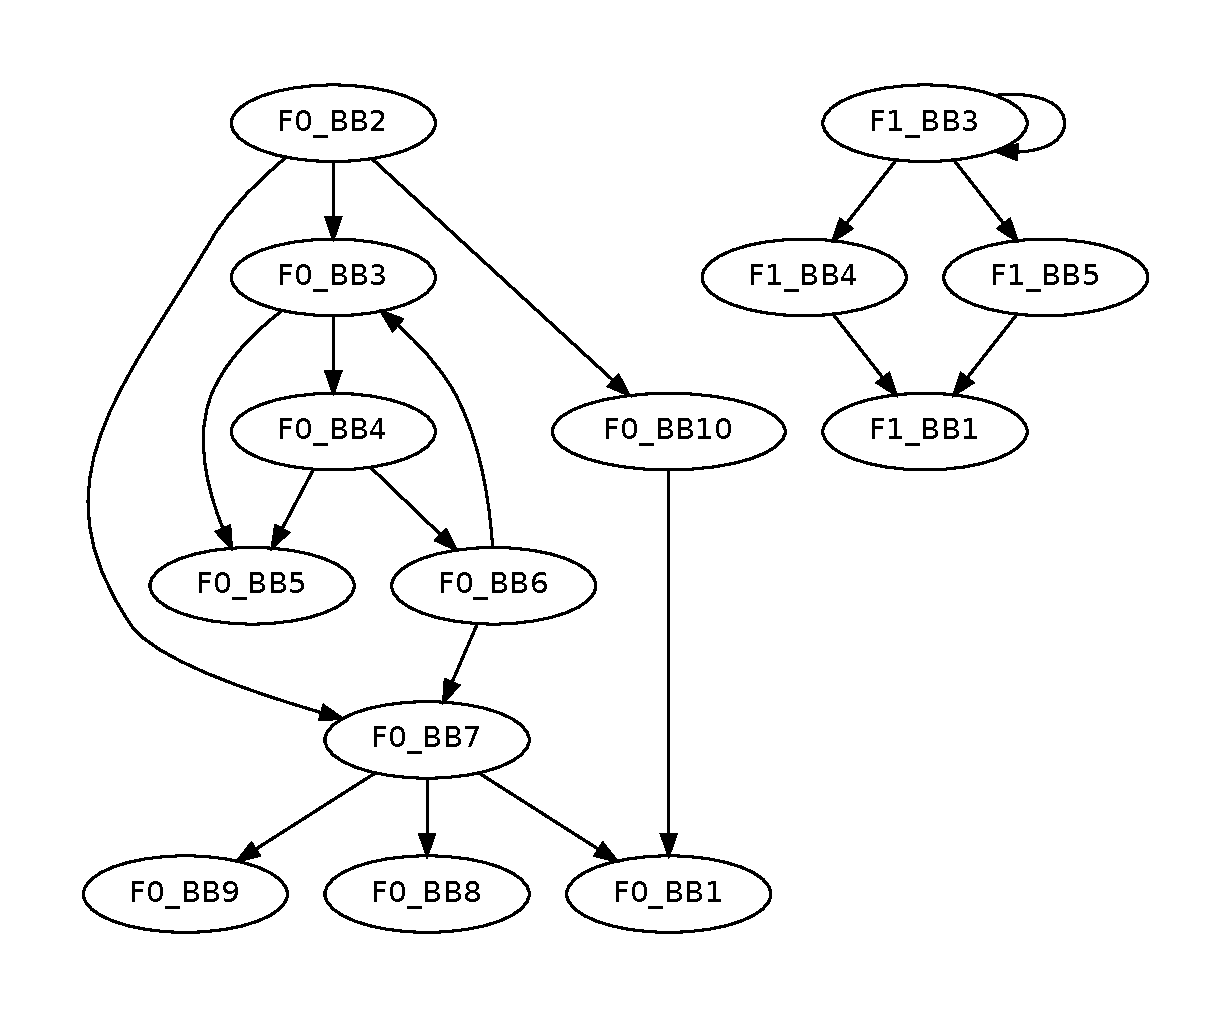
\includegraphics[scale=0.50]{images/t-test.pdf}
  \caption{Exemple de CFG d'une fonction}
  \label{fig:cfg}
\end{figure}
